%% Default Latex document template
%%
%%  blake@rcs.ee.washington.edu

\documentclass[letterpaper]{book}

% Uncomment for bibliog.
%\bibliographystyle{unsrt}
%
% \usepackage[T1]{fontenc}
% \usepackage{lmodern}
% \usepackage[utf8]{inputenc}
% \usepackage[english]{babel}
% \usepackage[pdftex,
%     pdftitle={ECE 474: Embedded Microcomputer Systems Course Notes},
%     pdfauthor={Blake Hannaford, University of Washington},
%     pdflang={en-US},
%     pdfsubject={ECE 474 Embedded Microcomputer Systems},
%     pdfkeywords={embedded systems, microcontrollers, ECE 474},
%     colorlinks=true,
%     linkcolor=blue,
%     urlcolor=blue,
%     citecolor=blue,
%     unicode]{hyperref}
% \usepackage{pdfcomment}
\usepackage{hyperref}
\usepackage{fancyhdr}
\usepackage{graphicx}
\usepackage{lineno}
\usepackage{listings}

%%%%%%%%%%%%%%%%%%%%%%%%%%%%%%%%%%%%%%%%5
%
%  Set Up Margins
\input{templates/pagedim.tex}

%
%        Font selection
%
%\renewcommand{\rmdefault}{ptm}             % Times
%\renewcommand{\rmdefault}{phv}             % Helvetica
%\renewcommand{\rmdefault}{pcr}             % Courier
%\renewcommand{\rmdefault}{pbk}             % Bookman
%\renewcommand{\rmdefault}{pag}             % Avant Garde
%\renewcommand{\rmdefault}{ppl}             % Palatino
%\renewcommand{\rmdefault}{pch}             % Charter


%%%%%%%%%%%%%%%%%%%%%%%%%%%%%%%%%%%%%%%%%%%%%%%%%
%
%         Page format Mods HERE
%
%Mod's to page size for this document
\addtolength\textwidth{0cm}
\addtolength\oddsidemargin{0cm}
\addtolength\headsep{0cm}
\addtolength\textheight{0cm}
%\linespread{0.894}   % 0.894 = 6 lines per inch, 1 = "single",  1.6 = "double"

% header options for fancyhdr

%\pagestyle{fancy}
%\lhead{LEFT HEADER}
%\chead{CENTER HEADER}
%\rhead{RIGHT HEADER}
%\lfoot{Hannaford, U. of Washington}
%\rfoot{\today}
%\cfoot{\thepage}



% Make table rows deeper
%\renewcommand\arraystretch{2.0}% Vertical Row size, 1.0 is for standard spacing)

\begin{document}

\title{--- ECE474 Notes Pack Spring 2026 ---}

\author{
        Blake Hannaford\\
        Department of Electrical \& Computer Engineering \\
        The University of Washington
}

%%%%%%%%%%%%%%%%%%%%%%%%%%%%%%%%%%%%%%%%%%%%%%
%
%  This uses the 'c' output stream from our SHN documents
%  Build this notes pack as follows:
%
%  1) run ./gen_tex_files to generate all the *.c.tex files
%     below
%  2) pdflatex (this file)
%
%  The command used by ./gen_tex_files is 
%    >coursetex --out c file.shn
%

\date{\today}

\maketitle

\tableofcontents

\chapter{Introduction}
    \input{474_IntroSp26.c.tex}
\chapter{C Program Structure}
    \input{Cprog.c.tex}
\chapter{Pointers}
    \input{Pointers.c.tex}
\chapter{Constants and Defines in C}
    %%%%%%%%%%%%%%%%%%%%%%%%%%%%%%%%%%%%%%%%%%%%%%%%%%%%%%
%%
%%           EE474 C constants and #define
%%
%%
%   % combined into notes pack
%
%\documentclass{article}
%\documentclass{seminar}
%
%\newpagestyle{BHstyle}{\sl U. of Washington \hfil EE 474 \hfil \thepage}{Hannaford \hfil \today}
%\pagestyle{headings}
%\slidepagestyle{BHstyle}
%\addtolength\oddsidemargin{3cm}
%\usepackage[T1]{fontenc}
%\usepackage[utf8]{inputenc}
%\usepackage[english]{babel}
%\usepackage{graphicx}
%\usepackage[pdftex,
%    pdftitle={ECE 474: C Constants and Preprocessor Directives},
%    pdfauthor={Blake Hannaford, University of Washington},
%    pdflang={en-US},
%    pdfsubject={ECE 474 Embedded Microcomputer Systems},
%    pdfkeywords={embedded systems, microcontrollers, ECE 474},
%    hidelinks,
%    unicode]{hyperref}
%\usepackage{listings}
%
%
%\oddsidemargin 0in
%\evensidemargin 0in
%\textwidth 6.5in
%\textheight 8.7in
%\topmargin 0.2in
%
%
%
%
%\linespread{1.0}
%
%
%\begin{document}
	%<*>
%\begin{slide}
\section*{{\tt C} Constants, Defines and Integers \footnote{
 B. Kernigan and D. Ritchie, ``The C Programming Language,,''
 2nd Edition, Prentice Hall, 1988.  \\
 Daniel W. Lewis, Fundamentals of
 Embedded Software, {\it Where C and Assembly Meet}, Prentice Hall, 2002.}
 }

%\end{slide}
%\begin{slide}

%%%%** Section 1 
\section{Review of C Constants}

We will often need to specify the content of memory
very precisely.

%%%%** Section 1.1
\subsection{HEX and OCTAL review}

	%<*chn>
Entering binary numbers can wear out the 1 and 0 keys on
your computer!   HEX is a good shorthand for binary since
each HEX character maps to a specific bit pattern.


\vspace{0.2in}	%<chn>
	%<*>
\begin{tabular}{|c|c|r|}
\hline
bits  &  HEX & Octal \\ \hline
0000  &  0   & 0     \\ \hline
0001  &  1   & 1     \\ \hline
0010  &  2   & 2     \\ \hline
...   &  ...    & ...      \\ \hline
0111  &  7   & 7     \\ \hline
1000  &  8   & 10     \\ \hline
1001  &  9   & 11     \\ \hline
1010  &  A   & 12     \\ \hline
1011  &  B   & 13     \\ \hline

...   & ...  & ...   \\ \hline
1111  &  F   & 17     \\
\hline
\end{tabular}

\vspace{0.2in}	%<chn>

Hex Place value: To convert {\tt 0xD2FB} to decimal:

%\vspace{0.2in}
\begin{tabular}{|c|c|c|c|}
\hline
D       &       2       &       F       &       B \\ \hline
$2^{12}$        &       $2^8$   &       $2^4$   &       $2^0$ \\ \hline
4096    &       256     &       16      &       1 \\ \hline
        &               &               &          \\ \hline
\end{tabular}
%\vspace{0.2in}

	%<*chn>
Octal
can also be used and is easier to memorize because there are
only 8 symbols (0-7). However, to fill
a byte of memory requires 2.5 octal characters since each
character only encodes 3 bits.  For example,
	%<*>

{\tt HEX 9A}  = Binary {\tt 1011010 } = Octal {\tt 132}

(Hex: 4-bit groups.   Octal: 3-bit groups)

%\end{slide}
%\begin{slide}


\begin{itemize}
  \item
  Ordinary numbers are interpreted by the C compiler
          as decimal values.   Example: {\tt 25 = 1101}

  \item Hex values are indicated to the C compiler by the
              prefix {\tt Ox} for example:   {\tt Ox2F}

  \item Octal values are indicated by a leading zero: {\tt 028}
            is a syntax error (why?).

\end{itemize}


%\end{slide}
%\begin{slide}

%%%%** Section 1.2
\subsection{Constant Syntax in C}

It is very important to use symbolic constants ({\tt \#define}'s )
for {\em all} your numeric constants.  Here are the
main reasons:
\begin{itemize}
        \item Code is more readable by humans.
        \item Code is much easier to change.
\end{itemize}

%%%%** Section 1.2.1 
\subsubsection{Example and Exercise}
	%<*chs>
{\small\tt
\begin{verbatim}
// Constants
#define EXAMPLE_CONST_D  1234 ;  /* DECIMAL value  */
#define EXAMPLE_CONST_H 0x4D2 ;  /* HEX value  */
#define EXAMPLE_CONST_O 02322  ; /* OCTAL value */

int x = EXAMPLE_CONST_D;
int y = EXAMPLE_CONST_H;
int z = EXAMPLE_CONST_O;

// test yourself here: (which of these print?)
if (x == y) printf ("Hello there ... \n");
else {};

if (y == 1234) printf ("What's up doc?? \n");
else {};

if (z == 2322)  printf ("The Rain in Spain  ... \n");
else {};

if (z = 2322)  printf ("Falls mainly on the plains.\n");
else {};

\end{verbatim}
}

%
%{\small\tt
%\begin{verbatim}
%// Constants
%#define EXAMPLE_CONST_D  1234 ;  /* DECIMAL value  */
%#define EXAMPLE_CONST_H 0x4D2 ;  /* HEX value == dec: 1234 */
%#define EXAMPLE_CONST_O 02322  ; /* OCTAL value */
%
%int x = EXAMPLE_CONST_D;
%int y = EXAMPLE_CONST_H;
%int z = EXAMPLE_CONST_O;
%
%// test yourself here: (which of these print?)
%if (x == y) printf ("Hello there ... \n");  **YES**
%else {};
%
%if (y == 1234) printf ("What's up doc?? \n");  **YES**
%else {};
%
%if (z == 2322)  printf ("The Rain in Spain  ...\n");  **NO**
%else {};
%
%if (z = 2322)  printf ("Falls mainly on the plains.\n");   **YES**
%else {};
%
%\end{verbatim}
%}
	%<*>


%\end{slide}
%\begin{slide}


%%%%** Section 1.2.2 
\subsubsection{Example 2}
Suppose you are going to control a CD-ROM drive and you want
to open and close the drive door.  The bit to open and close
the drawer is the 4th bit in a register located at address
{\tt 0x2DA}.  Let's say that to set that bit we use the function
\begin{verbatim}
IO_Register_Set([addr],[value])
\end{verbatim}
where {\tt [addr]}
is the bus address of the I/O register you want to manipulate
and {\tt [value]} is the bit pattern you want to put there.

It is ``technically'' correct to use the following code:
\begin{verbatim}
\\ open CD-ROM door
IO_Register_Set(0x2DA, 0x10) ;
\end{verbatim}


%\end{slide}
%\begin{slide}

	%<*cnh>
However, if we come back to that code later (1 week or 10 years)
we will not know what that statement does (or if the comment is
correct) without a lot of research.  Instead we use defines
for much better code as follows:
%Use {\tt\#define} compiler directives instead!
	%<*>
\begin{verbatim}

\\ (this part is in the preamble before "main ()"
\\  or in a special ".h" include file
#define  CD_ROM_CONTROL_REG  0x2DA
#define  CD_ROM_DOOR_OPEN    0x010

\\ .... skip to inside the code

\\ open CD-ROM door
IO_Register_Set(CD_ROM_CONTROL_REG, CD_ROM_DOOR_OPEN) ;

\end{verbatim}

Now, isn't that better?!!
%
It is a requirement of EE474 that
your code be written this way.
%
We will take off points for
any numberical constants in the main body of code.

%\end{slide}
%\begin{slide}

%%%%** Section 2 
\section{Bitwise vs. Logical Operators}

The familiar Boolean
operations {\tt\bf AND}, {\tt\bf OR}  and  {\tt\bf NOT}
are provided {\em two ways} in C.


%%%%** Section 2.1
\subsection{Logical Operators}

These work on {\em arithmetic } types or pointers.

\begin{tabular}{l p{1.5in} }

{\tt\bf True}           & a non zero value. \\

{\tt\bf False}          & zero.           \\

{\tt\bf \&\&}           & {\tt\bf AND}     \\

{\tt A \&\& B }         & True if {\it both} {\tt A} and {\tt B} are non-zero. \\

{\tt ||}                &  {\tt\bf OR} \\

{\tt A || B }           &  True if {\it either} {\tt A} and {\tt B} are non-zero.\\

{\tt ! }                &   {\tt\bf NOT} \\

\end{tabular}


%\end{slide}
%\begin{slide}

%%%%** Section 2.2
\subsection{Bitwise Operators}

A very important C feature for embedded microcomputer systems.
These operators are only defined for integer-like variables i.e.
{\tt char, short, int, and long} signed or unsigned.


\begin{tabular}{l l}
\&                      &       bitwise AND \\
\textbar                &       bitwise OR   \\
\textasciicircum        &       bitwise XOR  \\
\textless\textless      &       left shift   \\
\textgreater\textgreater&       right shift    \\
\textasciitilde         &       ones complement \\

\end{tabular}


%\end{slide}
%\begin{slide}

%%%%** Section 2.3
\subsection{Examples:}

{\tt
\begin{verbatim}

/* Use of bitwise logical operators  */

#define  Bit_Zero   0x01
#define  Bit_One    0x02
#define  Bit_Two    0x04
#define  Bit_Three  0x08
#define  Bit_Four   0x10
#define  Bit_Five   0x20
#define  Bit_Six    0x40

// etc etc etc ..


int x = 0x0B;           // x  = [... 0 0 0 0 1 0 1 1]

int y = 011;            // y  = [... 0 0 0 0 1 0 0 1]

int z = x << 2;         // z  = [... 0 0 1 0 1 1 0 0]

int z1 = y & Bit_Three; // z1 = [... 0 0 0 0 1 0 0 0]

int z2 = z | Bit_Four;  // z2 = [... 0 0 1 1 1 1 0 0]

\end{verbatim}
}


%\end{slide}
%\begin{slide}

\newpage	%<!s>
%%%%** Section 3 
\section{In-class Exercise:}

%
%\begin{verbatim}
%
%Convert 0x1A to decimal: __26_
%
%
%Convert 0xA2 to decimal:  __162____
%
%
%Convert 020 to Hex:    _____10_______
%
%
%Convert 0x20 to Octal: _____40_________
%
%\end{verbatim}
%
%{\tt
%\begin{verbatim}
%/* Give the binary value of the least significant
%8 bits of the following values:   */
%
%int aa = 0xC5;     // aa = [  1 1 0 0 0 1 0 1  ]
%
%int ab = 017 + 1;  // ab = [  0 0 0 1 0 0 0 0  ]
%
%int a = x | y;     // a  = [  0 0 0 0 1 0 1 1  ]
%
%int b = Bit_Two | Bit_Five | Bit_Seven;
%                   // b  = [  1 0 1 0 0 1 0 0  ]
%
%int c = ~((z | Bit_Zero) << 1);
%                   // c  = [  1 0 1 0 0 1 0 1 ]
%
%int d = !(z1 | Bit_Two);
%                   // d  = [  0 0 0 0 0 0 0 0 ]
%\end{verbatim}
%}
%
	%<*chs>

\begin{verbatim}

Convert 0x1A to decimal: __________


Convert 0xA2 to decimal:  __________


Convert 020 to Hex:  _____________________


Convert 0x20 to Octal: _____________________

\end{verbatim}

{\tt
\begin{verbatim}
/* Give the binary value of the least significant
8 bits of the following values:   */

int aa = 0xC5;     // aa = [                     ]

int ab = 017 + 1;  // ab = [                     ]

int a = x | y;     // a  = [                     ]

int b = Bit_Two | Bit_Five | Bit_Seven;
                   // b  = [                     ]

int c = ~((z | Bit_Zero) << 1);
                   // c  = [                     ]

int d = !(z1 | Bit_Two);
                   // d  = [                     ]
\end{verbatim}
}

	%<*>
\newpage	%<!s>
%%%%** Section 4 
\section{Binary Integers}

%%%%** Section 4.1
\subsection{Unsigned Integer}

Typically just a
16 bit binary number.  Straightforward, but cannot represent
negative numbers.

If {\tt x } is of type {\tt unsigned int}, then
\[
0 \leq {\mathtt x} \leq 65535
\]


%\end{slide}
%\begin{slide}

C declaration of unsigned integers:

\begin{verbatim}
unsigned char a,b;            // 8 bit unsigned
unsigned int  x,y,z;          // 16 bit unsigned
unsigned long int p,q,r;      // 32 bit unsigned
\end{verbatim}



%\end{slide}
%\begin{slide}

%%%%** Section 4.1.1 
\subsubsection{Exercise}

Write a C function using bitwise logical operators etc. to print
the binary value of a 16 bit word.

\vspace{4in}	%<cn>

%\end{slide}
%\begin{slide}

%\vspace{3.0in}
%
%\begin{verbatim}
%void bin_display(unsigned int x)
%{
%        unsigned int i,j;
%        for(i=0;i<16;i++)
%        {
%                j = 1<<(15-i);
%                if(j & x) printf("1");
%                else      printf("0");
%        }
%}
%
%\end{verbatim}
%
%\end{slide}
%\begin{slide}
%
	%<*>
%%%%** Section 4.2
\subsection{2's Complement Integers}
	%<*chn>
Most common way to represent integers which can have both positive and negative
values.   Most significant bit (MSB) is the ``sign bit'' 0=positive, 1=negative.
however, if MSB is 1, other bits are subject to ``2's complement''.
%
%\begin{itemize}
%        \item MSB is ``sign bit'' 0= positive, 1=negative
%        \item if sign bit is 1, rest of word is in ``2's complement''
%\end{itemize}
%
	%<*>

To convert a number to or from two's complement,
\begin{enumerate}
  \item complement all bits
  \item add 1
\end{enumerate}
Taking the 2's complement of the entire $n$ bits is equivalent to negation.

For an $n$ bit number, $x$,  the range of all possible integers in 2's complement is
\[
-2^{n-1} \leq x \leq (2^{n-1}-1)
\]
(see Lewis Figure 2-4, page 22 for a useful chart).

%\end{slide}
%\begin{slide}

%%%%** Section 4.2.1 
\subsubsection{Exercise}

Write a c code fragment which negates a signed (2's complement) integer
using bitwise logical operators and addition.  Include declarations for
your variables.
(do not just multiply by -1)


\vspace{3.0in}	%<hc>

%\end{slide}
%\begin{slide}
%
%\begin{verbatim}
%
%[blake@alec code]$ cat twocomp.c
%/* twocomp.c
% *
% *  Demonstrate 2's complement
% *
% */
%void bin_display(unsigned int x);
%main(argc,argv)
%int argc;
%char *argv;
%{
%        int  a = -23;
%        int  b;
%        int i,j;
%        printf(" Decimal: %d \n    Binary:     ", a);
%        b = a;
%        bin_display((unsigned int)b);
%        printf("\n    Complement: ");
%        b =   ~a;     // complement all bits
%        bin_display((unsigned int)b);
%        printf("\n1 + Complement: ");
%        b = 1 + ~a;     // complement all bits and add 1
%        bin_display((unsigned int)b);
%        printf("\n Compare: %d %d\n", a, -b);   // should be the same
%}
%
%
%\end{verbatim}
%\end{slide}
%\begin{slide}
%%%%%** Section 4.3
%\subsection{Test Run}
%\begin{verbatim}
%
%[blake@alec code]$ ./twocomp
% Decimal: -23
%    Binary:     1111111111101001
%    Complement: 0000000000010110
%1 + Complement: 0000000000010111
% Compare: -23 -23
%[blake@alec code]$
%
%\end{verbatim}
%
%\end{slide}
%\end{document}
%

\chapter{Tasks and Schedulers}
    \input{Schedulers_Pt01.c.tex}
    \input{Schedulers_Pt02.c.tex}
\chapter{Scheduler Implementation}
    %%%%%%%%%%%%%%%%%%%%%%%%%%%%%%%%%%%%%%%%%%%%%%%%%%%%%%
%%
%%           EE474 Scheduler Implementation
%%
%   % combined into notes pack
%
%\documentclass{article}
%\documentclass{seminar}
%
%\newpagestyle{BHstyle}{\sl U. of Washington \hfil EE 474 \hfil \thepage}{Hannaford \hfil \today}
%\pagestyle{headings}
%\slidepagestyle{BHstyle}
%\addtolength\oddsidemargin{3cm}
%\usepackage[T1]{fontenc}
%\usepackage[utf8]{inputenc}
%\usepackage[english]{babel}
%\usepackage{graphicx}
%\usepackage[pdftex,
%    pdftitle={ECE 474: Scheduler Implementation},
%    pdfauthor={Blake Hannaford, University of Washington},
%    pdflang={en-US},
%    pdfsubject={ECE 474 Embedded Microcomputer Systems},
%    pdfkeywords={embedded systems, microcontrollers, ECE 474},
%    hidelinks,
%    unicode]{hyperref}
%\usepackage{listings}
%
%
%\oddsidemargin 0in
%\evensidemargin 0in
%\textwidth 6.5in
%\textheight 8.7in
%\topmargin 0.2in
%
%\title{Scheduler Implementations\\ECE/CSE474}
%
%\linespread{1.0}
% 
%
%
%\begin{document}
%
%
%\begin{slide}
%\maketitle
%
%
%%%%%** Section 1 
\section{How to Build a Scheduler}	%<schn>
%Up till now we have used a very simple loop such as 
%\begin{verbatim}
%while(1)
%  {
%  taskA();
%  taskB();
%  taskC();
%  time_delay();
%  }
%\end{verbatim}
%\end{slide}
%\begin{slide}
%
	%<*chn>
To make a very basic non-premptive, round-robin scheduler.   We can call this a {\it static} scheduler because the order of the task execution will never change. 
In this section we will expand our basic scheduler to give it some new features: 

%\subsection*{New features}
	%<*>
\begin{itemize}
  \item The ability of a task to halt itself.
  \item The ability of a task to sleep for a while.
\end{itemize}

%\end{slide}
%\begin{slide}

%%%%** Section 1.1
\subsection{Part I   Using function pointers to start a task}

Throught the course we are using the terms ``task" and ``function" almost interchangably.    This is because we implement our tasks with C functions. 	%<*chn>
How can we manipulate these functions so that they do not nescessarily execute in a fixed order?  

%\end{slide}
%\begin{slide}

	%<*>
We learned that the syntax:

\begin{verbatim}
type (*name)(type arg1, type arg2, ...)
\end{verbatim}
indicates a function pointer called {\tt name} which can point to any function having the same prototype.   For example

\begin{verbatim}
int (*fp)(char x, int y, double z)
\end{verbatim}

creates a function pointer {\tt fp} which can point to any function which returns an {\tt int} and has three arguments which are {\tt char, int, double} respectively.  With function pointers we can write code that can start an arbitrary function.   For example:	%<*chn>

%\subsection*{Example: start function}
	%<*>
\begin{verbatim}

void start_function(void (*functionPTR)() )
  {
     functionPTR();
  }

\end{verbatim}


%\end{slide}
%\begin{slide}

Now our basic scheduler could be written:

\begin{verbatim}
while(1)
  {
  start_function( taskA);
  start_function( taskB);
  start_function( taskC);
  time_delay();
 }
\end{verbatim}

but this is still kind of a trivial re-write of our basic loop above.   

%\end{slide}
%\begin{slide}

%%%%** Section 1.2
\subsection{Part II   Keeping lists of functions }

	%<*chn>
For our scheduler to be smarter than the basic {\tt while(1)} loop, we need to be able to put functions into lists.   That way we can keep track of which functions are ready, 
waiting, and inactive.    One approach would be a single list of tasks, with a corresponding array of integers to determine which state the task is in. 
Although logically OK. This approach is not preferred at this point, because the scheduler will have to do a lot of looking through the list to find which tasks are in a certain state.  

%\end{slide}
%\begin{slide}

	%<*>
We can create an array of function pointers as follows:

\begin{verbatim}
#define  NUMBER_OF_FUNCTIONS     10

void (*list_of_functions[NUMBER_OF_FUNCTIONS])(void *p)
\end{verbatim}

{\bf Example: }

\begin{verbatim}
#define  NT_RUNNING     10
void (*runningTasks[NT_RUNNING])(void *p)
\end{verbatim}
\noindent
... a list of all the tasks  which are currently running.  
We can use a {\tt NULL} pointer 
at the end of the list if there are less than {\tt NT\_RUNNING} active tasks 
(similar to the zero byte at the end of a string). 

%\end{slide}
%\begin{slide}

	%<*chn>
In the example above we created an  array which could hold 10 function pointers.  Each function pointer in the array must point to a function with the prototype:

\begin{verbatim}
void function(void *p)
\end{verbatim}
This is a good prototype for tasks because they do not need to return a value and the  {\tt void } pointer parameter is a flexible way to pass a parameter to a task that is being created (although we will not use this much).
 
	%<*>
Here then is some pseudocode for a main program and scheduler function:
 
\begin{verbatim}
//function prototypes for tasks
void taskA(void *p);
void taskB(void *p);
...

// function prototype for scheduler
void scheduler();


#define NTASKS     4

//lets make the task list global
 // an array of function pointers,
 // each one has a void* parameter.
 void (*readytasks[NTASKS]) (void *p);   

main()
   { 
   // initialize array of pointers to tasks
  readytasks[0] = taskA;
  readytasks[1] = taskB;
  ...
  // NULL signals the last task in the list.
  readytasks[3]= NULL;
 // now start scheduler
  while(1) {
      scheduler();
      time_delay();  // timer for 1ms loop time
     }
 } // end of main
\end{verbatim}

%\end{slide}
%\begin{slide}

	%<*chn>
Here, we have set up an array to contain pointers to the task as a global variable (so that it will be visible to both main and the scheduler function (not shown). 
Then, inside {\tt main()}, we have initialized each element of the array to point to one of our tasks.   The scheduler function will do the following (pseudocode)

%\subsection*{Scheduler function (pseudocode)}
	%<*>
\begin{verbatim}
scheduler() {
  if(readytasks[task_index] == NULL && task_index != 0) 
        { task_index=0; }
  if(readytasks[task_index] == NULL && task_index == 0){
             // figure out something to do because 
             // there are no tasks to run!
             }
  start_function(readytasks[task_index]);
  task_index++; // Round Robin/we're taking turns
  return;
 }
\end{verbatim}

%\end{slide}
%\begin{slide}

%%%%** Section 1.3
\subsection{part III  Manipulating the Task Lists}

	%<*chn>
So far, we have just made a more complicated form of our basic {\tt while(1) } loop scheduler.  Now let's allow tasks to halt themselves by calling a function called
{\tt halt\_me()}.   
First, we need to generate a second list for the tasks which might be halted.     Let's call it {\tt haltedtasks[]}.   Now, the scheduler can work as before, but when 
a task calls {\tt halt\_me()}, the following things have to happen:

%\subsection*{{\tt halt\_me} function}
	%<*>
\begin{verbatim}
halt_me() {
   * identify which task is currently running 
              (i.e. look at task_index)
   * copy the function pointer from readytasks[task_index] 
              to the haltedtasks array
   * move the remaining tasks up in readytasks[] to fill 
              the empty hole and copy NULL into the last 
              element.
   * increment the index of the haltedtasks array.
   * return;
  }
\end{verbatim}

%\end{slide}
%\begin{slide}

%
%When {\tt halt\_me} returns to the task, the task should {\tt return} and then it will not be started again by the scheduler since the current task has been deleted from 
%{\tt readytasks}.  But note, to make sure the program logic is correct, a task which wants to
%halt itself must add the {\tt return} after using {\tt halt\_me() }:
%
%Watch out for potential logic bug!
	%<*>
\begin{verbatim}

if (time_to_halt) {
     halt_me();
     return;
     }
     
\end{verbatim}

%
%because otherwise the task will run its course after {\tt halt\_me()} until it eventually encouters {\tt return}.
	%<*>

%\end{slide}
%\begin{slide}

\subsection*{Sleep}

	%<*chn>
  Now let's try to set up a {\tt Sleep(int d)} function which can let our tasks
go to sleep for {\tt d} msec.   Just like with {\tt halt\_me()},
we need to call {\tt return} after {\tt sleep()}. 
A function which wants to sleep will have to
look like:

	%<*>
%\subsection*{Typical Task using sleep()}
\begin{verbatim}
task_c(p) {
   compute for a while;
   if(its_bed_time){
        sleep(10);
        return;
        }
    else {
        do some more computing;
        }
    return;
   }
\end{verbatim}

	%<*chn>
We will impose the requirement that the new {\tt sleep(d)} function will not put the task to sleep until the task that called it has {\tt return}ed.    How would the scheduler work now?
As above, we need to generate a new list for tasks which are waiting for time delays.   Lets call it {\tt waitingtasks[]}.   Then we also have to make an array for 
the time delays for each waiting task.    When a function calls {\tt sleep(d)} the following things should happen

%\end{slide}
%\begin{slide}

	%<*>
\subsection*{Sleep function (pseudocode)}
\begin{verbatim}
sleep(int d) {
  * copy function pointer from readytasks[task_index] 
          to the waitingtasks[] array. 
  * clean up readytasks[] as in halt_me();
  * copy d into the delays array with the same index 
          as the function pointer has in waitingtasks[]
  }
\end{verbatim}

	%<*chn>
Now the scheduler must keep track of waiting times for any tasks which are sleeping and  wake them up  by moving them back to the {\tt readytasks[]} array at the right time.
Let's add some pseudocode to the bottom of the scheduler function above:

%\end{slide}
%\begin{slide}
	%<*>
%\subsection*{Keeping track of sleep delays}
\begin{verbatim}
...
* for each element of waitingtasks which is not NULL:
      decrement the delay value d.
      if (d==0) move the function pointer to the end
            of the readytasks[] array and remove it 
            from waitingtasks.
// end of scheduler
  return;
}
\end{verbatim}
 

%\end{slide}
%\begin{slide}

	%<*>
%%%%** Section 1.4
\subsection{An Alternate Data Structure for Scheduling}
	%<*chn>
So far we have used arrays of function pointers to keep track of the tasks in each state.  We also used an array of delay values for the remaining delay of sleeping tasks.   Another approach is to keep everything about the task in a struct and then manipulate the structs to change task states.  We call such structs {\bf Task Control Blocks (TCB's)}.   For example, we could define the TCB as follows:
% Let's set up a struct which contains everything we need to track about a Task:
	%<*>
\begin{verbatim}
typedef struct TCBstruct {
    void (*ftpr)(void *p);     // the function pointer
    void *arg_ptr;             // the argument pointer
    unsigned short int  state;  // the task state
    unsigned int delay;        // sleep delay
    } ;
\end{verbatim}

	%<*chn>
Now we have a single place that stores everything about a task.  Now we can set up an array of {\tt tcb}'s to hold all tasks and define constants for the states:

%\end{slide}
%\begin{slide}

	%<*>
\begin{verbatim}
#define  STATE_RUNNING   0
#define  STATE_READY     1
#define  STATE_WAITING   2
#define  STATE_INACTIVE  3

TCBStruct TaskList[N_MAX_TASKS];
\end{verbatim}

Then we can set up the task list as follows:

\begin{verbatim} 
int j=0;
int task_B_Arg;

TaskList[j].ftpr = task_A();
TaskList[j].arg_ptr = NULL; 
TaskList[j].state = STATE_INACTIVE;
TaskList[j].delay = -1;
j++;

TaskList[j].ftpr = task_B();
// (example: let's say we need an arg value of 56)
task_B_Arg = 56;    
int *ip = &task_B_Arg;
TaskList[j].arg_ptr = (void*)ip; 
TaskList[j].state = STATE_READY;
TaskList[j].delay = -1;
j++;

TaskList[j].fptr = NULL;  // marks end of list

... maybe other tasks  ...
\end{verbatim}

	%<*chn>
We have initialized the scheduler with two tasks, A and B.  Their information goes into the first two entries in {\tt TaskList[]}.   Task A has no argument (more precisely the single void pointer argument will not be used), and starts out in {\tt STATE\_INACTIVE}.   This means that it will have to be started by some other task.   In this example, we want to start task B with an argument of 56, so we set an integer to 56, make a pointer which points to it, and then cast it to {\tt void*} before assigning it to the {\tt arg.ptr} member.   We might want Task B to start right up so Task B starts in {\tt STATE\_READY} to
go into the CPU as soon as possible.   The next element of {\tt TaskList[]} is set to NULL which will be our signal for no more tasks. 

Now, {\tt halt\_me()} just has to figure out which element of {\tt TaskList[]} it currently belongs to and change its state from {\tt STATE\_RUNNING} to {\tt STATE\_INACTIVE}.   Similarly, if Task B called a function to {\tt start} Task A, then that function would just have to change Task A's state from {\tt STATE\_INACTIVE} to {\tt STATE\_RUNNING}.
%\end{slide}
%\begin{slide}
	%<*>
\subsubsection*{In Class Exercise: Starting, Stopping, Delay}
 Write pseudocode for {\tt halt\_me()}, {\tt start\_task(int task)},  and {\tt delay(int d)} a task.  
 
 Assume that TCBs have been set up already as above.
 
 Assume {\tt t\_curr} is an integer which points to the currently running task.
 
\vspace{0.5in}
{\bf (solution on next slide!) }

\vspace{5.0in}	%<ch>
%\end{slide}
%\begin{slide}
%
%\begin{verbatim}
%halt_me() {
%    TaskList[t_curr].state = STATE_INACTIVE;
%    }
%
%start_task(int task_id) {
%    TaskList[task_id].state = STATE_READY;
%    }
%
%delay(int d) {
%    TaskList[t_curr].delay = d;
%    TaskList[t_curr].state = STATE_WAITING;
%    }
%\end{verbatim}
%
%
%\end{slide}
% \end{document}
%

\chapter{Embedded System Hardware and I/O}
    \input{Hardware_IO.c.tex}
\chapter{Interrupts}
    %%%%%%%%%%%%%%%%%%%%%%%%%%%%%%%%%%%%%%%%%%%%%%%%%%%%%%
%%
%%           EE474 Hardware and Basic I/O
%%
%   % combined into notes pack
%
%\documentclass{article}
%\documentclass{seminar}
%
%\newpagestyle{BHstyle}{\sl U. of Washington \hfil EE 474 \hfil \thepage}{Hannaford \hfil \today}
%\pagestyle{headings}
%\slidepagestyle{BHstyle}
%\addtolength\oddsidemargin{3cm}
%\usepackage[T1]{fontenc}
%\usepackage[utf8]{inputenc}
%\usepackage[english]{babel}
%\usepackage{graphicx}
%\usepackage[pdftex,
%    pdftitle={ECE 474: Interrupts},
%    pdfauthor={Blake Hannaford, University of Washington},
%    pdflang={en-US},
%    pdfsubject={ECE 474 Embedded Microcomputer Systems},
%    pdfkeywords={embedded systems, microcontrollers, ECE 474},
%    hidelinks,
%    unicode]{hyperref}
%\usepackage{listings}
%
%
%\oddsidemargin 0in
%\evensidemargin 0in
%\textwidth 6.5in
%\textheight 8.7in
%\topmargin 0.2in
%
%
% 
%\linespread{1.0}
%
	%<*>
%\begin{document}
%\begin{slide}

%%%%** Section 1 
\section{Process Context}
%%%%** Section 1.1
\subsection{What is context?}
A process is sometimes called a task, subroutine or
program.  Process {\bf context} is all the information that
the process needs to keep track of its state.

\begin{description}
\item[Registers]   Temporary storage locations for a few
bytes.  Typical CPU has 8-64 registers.
\item[Program Counter] A special register which points to the
next instruction to be executed.
\item[Stack Pointer] Another special register which points to
the top (bottom) of a stack of data
\item[Processor Flags] Hardware bits in the CPU which detect
errors or arithmetic results.
\end{description}

Sometimes also called ``processor state''.

Example:  reading a book and the phone rings.

%\end{slide}
%\begin{slide}

%%%%** Section 1.2
\subsection{Context Switching}

When we call a subroutine (function) or when an
interrupt happens, we need to {\bf save} the current context
because we are starting a new one.

This happens a lot so it must be efficient.


\begin{itemize}
         \item After function completes, must know where to resume.
         \item New process can mess up information in old process.
        (i.e. what if they both use the same register?)
        \item Saving the context and restoring it is called
        {\bf context switching}.
\end{itemize}


%\end{slide}
%\begin{slide}

Procedure: To switch contexts from Process 1 to Process 2:
\begin{enumerate}
\item Control is passed from Proc1 to ``OSH"
\item OSH saves processor state from CPU registers(immediately!)
\item OSH finds stored state of Proc2 and restores it
into CPU registers.  IR is restored last.
\item CPU jumps to Proc1 code according to IR.
\end{enumerate}
{\bf OSH = Operating System or Hardware.}

%\end{slide}
%\begin{slide}

%%%%** Section 1.3
\subsection{Types of Context Switches}

\begin{itemize}
\item Subroutine Call. Either to user routine or to OS.
\item Interrupt.  Hardware initiated context switch.
\end{itemize}


%\end{slide}
%\begin{slide}

%%%%** Section 1.4
\subsection{Calls}

\begin{itemize}
\item User subroutine (e.g. {\tt sin($\theta$)}  ).  \\
  Main program context is saved, {\tt sin($\theta$)} routine is loaded.
\item System Calls Examples
        \begin{itemize}
        \item I/O such as write block of data to disk
        or apply a value to D/A converter.
        \item Process Control:  halt, wait (pend),
        start, kill, or unblock another process.
        \item Interprocess Communication:  pipes,
        mailboxes, semaphores.
        \item Return from Interrupt.
        \end{itemize}


\end{itemize}

%\end{slide}
%\begin{slide}

%%%%** Section 1.5
\subsection{The Stack}
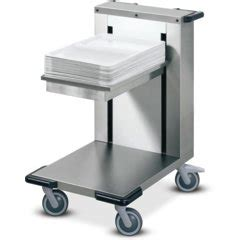
\includegraphics[width=2in]{misc_figs/traystack.png}\\
\noindent
Did your school cafeteria have one of these?\vspace{0.2in}

Problem:  How to allocate space for context storage. Consider
nesting of subroutine calls.
Solution: A stack is a data structure modeled on a spring-loaded cafeteria stack.

\begin{itemize}
        \item {\bf Push:} a piece of information on the stack.
        \item {\bf Pop: } a piece of information off of the stack.
        \item Always put/take info from current stack top.
\end{itemize}



Stacks are implemented with a {\bf Stack Pointer}.
 Enter the proper C code on the blank lines according	%<ch>
 to class discusion.	%<ch>

\begin{itemize}

% \item {\bf Push:} {\tt (*SP--) = piece\_of\_information}
 \item {\bf Push:} {\tt \_\_\_\_\_\_  =piece\_of\_information}	%<ch>
% \item {\bf Push:} {\tt *(SP--) =piece\_of\_information}

% \item {\bf Pop:}  {\tt SP++ ; piece\_of\_information = *SP }
 \item {\bf Pop:}  {\tt piece\_of\_information = \_\_\_\_\_\_ }	%<ch>
% \item {\bf Pop:}  {\tt SP++ ; piece\_of\_information = *SP }

        \item {\bf Initialize Stack:} {\tt SP = stack\_top}
        \item Stack grows down.
        \item Have to allocate space for maximum stack depth.
\end{itemize}


%\end{slide}
%\begin{slide}

%%%%** Section 1.6
\subsection{Subroutine Call}
How to call a subroutine (function in C).
(the compiler generates instructions to do all this
so you don't have to!)
\begin{enumerate}
        \item Push i argument {\it values} to stack: \\
% <s>                {\tt foreach {i} (*SP)-- = argument(i);}
                {\tt foreach {i} \_\_\_\_\_\_ = argument(i);}
% <n>                {\tt foreach {i} *(SP--) = argument(i);}
        \item Generate {\tt JSR} machine instruction.
        \begin{enumerate}
                \item Push machine registers onto stack.
                \item Load subroutine addr into PC
                \item execute next instruction (i.e. jump to
                *PC).
        \end{enumerate}
        \item Subroutine looks for arguments at {\tt
                *(SP - MACH\_REG\_SIZE) }
        \item When Subr. completes, execute {\tt RET} instruction.
        \begin{enumerate}
                \item Pop machine registers from stack.
                \item Clean up stack from function args:
                {\tt foreach {i} SP++;}
                \item Load old value into PC
                \item execute next instruction (i.e. jump to
                *PC).
        \end{enumerate}



\end{enumerate}

%%%%** Section 2 
\section{Interrupts}

An interrupt stops whatever instruction sequence is being executed by the processor and starts
some new code.  This happens in response to a specific hardware event event (the ``Interrupt") which 
could be internal or external.  The purpose of the new code is to immediately perform tasks 
specifically related to the event.   Let's look at some common terms used with interrupt programming.

\subsection{Interrupt Definitions}

{\bf Interrupt Service Routine (ISR):} When an interrupt is generated, some code, 
called an ISR, must be run immediately to “service” the interrupt.   ``Service"
means to perform tasks needed by the event that caused the interrupt.   For an 
extremely simple example, if a timer is causing regular clock interrupts, an ISR 
might just increment a variable called “time” and return.  A more advanced 
example would be a disk drive which earlier got a command to read data from a 
hardware disc sector.    After the sector read is completed, the drive generates 
an interrupt, and the ISR must grab the data from the drive and put it into the 
right place in memory. 

{\bf Enabling interrupts:  } Just like when you concentrate on some reading or 
writing task, interruptions are costly for the CPU.  Furthermore, if there is no 
ISR defined for the interrupt, then acting on that interrupt could hang (freeze) 
the system.   Therefore there are bits controlled by software that enable or 
disable interrupts from hardware signals.   By default all the interrupts are 
disabled.    In addition to enabling individual interrupts, the CPU has bits 
that can globally enable or disable all interrupts.

{\bf Internal Interrupts:} Interrupts from components inside the computer itself such as timer/counters. 

{\bf External interrupts: } Interrupts from components outside the CPU such as a digital input bit, a network interface, or an SSD.

{\bf Interrupt Priorities:}   Interrupts can interrupt ISRs(!)  ... or not!    You might have one interrupt which is a very time-critical control function, and a plane will crash if this ISR does not execute correctly in 2milliseconds.   You might also have another ISR that updates a log file.   The first ISR is therefore a much higher priority than a log-file update.   Yes, we need to guarantee that the log file gets updated, but the speed does not matter.    Most processors group the available interrupts into priority levels such that lower priority interrupts have to wait until there are no running ISRs of higher priority. 

{\bf Interrupt Vectors: }    A powerful computer system could have many different interrupts that are enabled at a given time.   A simple example would be a Network-Attached-Storage (NAS) device which is basically a computer with a bunch of disk drives (or SSDs) attached to it to be a file server.    If there are four drives attached to the NAS, each one needs a separate interrupt so that they can operate simultaneously.   The way to implement this is for each hardware interrupt mechanism to have a pointer to a software ISR function.    The address of the ISR for each interrupt is the “Interrupt Vector”.  

{\bf Interrupt Vector Table:}  This is a hardware-specific region of memory that is specially set aside (and hardware-defined) to hold an interrupt vector for each hardware interrupt the processor can support.   If the interrupt is not enabled then it doesn’t matter what is in the table, but for every enabled interrupt, there must be a valid pointer to a function that can run and return. 
 

Types of inputs that can cause an interrupt:
\begin{itemize}
        \item User pushes a button or moves a mouse.
        \item Packet arrives on network interface.
        \item A sensor detects an event.
        \item Disk drive
 completes an operation and has a bunch of data ready for CPU.	%<chn>
        \item A clock
 can be programmed to set up interupts at regular intervals.	%<chn>
        \item A hardware timer
 can count clock pulses and generate an interrupt when it gets to zero.	%<chn>
        \item A thermostat
 indicates that a temperature setpoint is reached.	%<chn>
\end{itemize}


\paragraph{Connections}

Interupts are logic signals physically wired to the CPU
(or interrupt processor peripheral).	%<chn>

There are various schemes for wiring multiple interrupts:

\paragraph{Priority}

\begin{itemize}
        \item 7 lines leading into CPU.
        \item peripherals can pull one line low
 for example using open collector ``wired OR''.	%<chn>
        \item A small address bus identifies the specific
        interrupt within a line.
        \item Lines are ranked by priority
 e.g. ISR for Line 0 cannot be interrupted by any other interrupt,	%<chn>
ISR for Line 6 can be interrupted by ANY other interrupt.	%<chn>
\end{itemize}

\paragraph{Interrupt Vectors}

Each interupt has a specific code number which is applied to
the processor interrupt address bits (maybe 8bits).

CPU has a specific hard-wired memory address called the
{\bf interrupt vector table.}    The interrupt vector
table is an array of function pointers.  The functions
they point to are called
{\bf interrupt service routines, ISRs}.

\paragraph{Typical Interupt Vector Table}
{\tt
\begin{tabular}{|r|r|}
\hline
Memory Addr             &       Contents \\ \hline

1000                    &       isr\_0()  \\ \hline
1002                    &       isr\_1()  \\ \hline
1004                    &       isr\_2()  \\ \hline
1006                    &       isr\_3()  \\ \hline
...                     &       ...       \\ \hline
1100                    &       isr\_N()  \\ \hline

\end{tabular}
}

\paragraph{Meaning of ISRs}

Each hardware device is hooked up to a specific interrupt vector
table address.  We need to write each ISR to handle the proper
device.

%%%%** Section 2.1
\subsection{ISRs}

\paragraph{Servicing an interrupt}

\paragraph{Hardware Level}

 The hardware does the following steps when an interupt	%<chn>
is detected:	%<chn>

% Upon hardware interrupt:
\begin{enumerate}
        \item Push processor context onto stack.
        \item Load appropriate address from IVT into
        program counter (PC).
        \item jump to *PC.
\end{enumerate}

\paragraph{Software Level}

 The ISR is now in control.  The ISR must do the	%<chn>
 following.	%<chn>

\begin{enumerate}
        \item (There are no arguments)
        \item block (``mask'') all other interrupts if necessary
        \item ``service'' the device.
        \item unmask other interrupts
        \item  Execute a return from interrupt instruction
\end{enumerate}

\paragraph{Hardware Level}

Now the hardware takes over again to clean up the interrupt.	%<chn>

\begin{enumerate}
        \item Pop processor context from the stack.
        \item Last item is PC
        \item continue whatever was being done when interrupt
        occured.
\end{enumerate}


%\end{slide}
%\begin{slide}

%%%%** Section 2.2
\subsection{ISR Programming}

 Some tips for successful ISR programming	%<chn>

\paragraph{Problems with ISRs}
\begin{itemize}
        \item ISRs are virtually impossible to debug!
        \item The debugger uses ``software interrupts'' to handle
        tricks like breakpoints and single stepping.
        \item thus even correct ISRs will break the debugger OR
        \item the debugger will break your ISRs
        \item ISRs take over the processor -- even pre-emptive
        schedulers.
        \item ISRs can easily mess up other processes if they

                \begin{itemize}
                \item write in wrong global variables
                \item take up a lot of CPU time
                \item play around with the stack
                \end{itemize}
\end{itemize}


%\end{slide}
%\begin{slide}

\paragraph{ISR Solutions}


\begin{itemize}
        \item Keep your ISRs  {\it small, simple, \& quick }
        \item No loops inside ISR's
        \item No complex logic (no nested {\tt if}'s )
        \item Don't do unrelated I/O in the ISR (for example,
        no {\tt printf("ISR message");}).
        \item Guidelines: Max: 1/2 page of C, 1 page of ASM
        \item Do not trust / use debugger.
        \item Do absolute minimum of stuff in ISR, do the
        rest in a regular task.
        \item Check and recheck your use of interrupt masking
        and how you save and restore the context.

\end{itemize}


%\end{slide}
%\begin{slide}
%%%%** Section 3 
\section{Real Time Control }

%%%%** Section 3.1
\subsection{Basic Task}
Map inputs to outputs (through a control law) at
{\it regular } time intervals.


%\end{slide}
%\begin{slide}

\begin{verbatim}
\% Initialization
set_up(timer0);
set_up(input,output);

\% endless control loop
while(1)
        {
        wait(timer0);
        x=read(input);
        y=control_function(x);
        output(y,output);
        }
\end{verbatim}

%\end{slide}
%\begin{slide}

%%%%** Section 3.2
\subsection{Timing}
Different ways to ensure regular time sampling.


\begin{itemize}
        \item While loop + Interrupt
        \begin{itemize}
                \item ``main" program is {\tt while(1);}
                \item Timer is set up for regular interrupts
                every {\tt T} seconds.
                \item ISR is I/O and control law: \\
                {\tt x=read(input); \\
                y=control\_function(x);  \\
                output(y,output); \\
                return();}
        \end{itemize}
%\end{itemize}

%\end{slide}
%\begin{slide}

%\begin{itemize}
        \item  ``spin-lock'': \\
         {\tt wait(timer0) $\to$ while(timer0 == 0) ;}
        \item  OS Call:   \\
        {\tt wait(event)} \\
        return control to OS until {\bf event} occurs.  {\bf event} is timer0.
\end{itemize}




%\end{slide}

%\end{document}

\chapter{Serial Communication}
    \input{Serial.c.tex}
% \chapter{TCP/IP and Socket Communciation}
%     \input{Tcpip.c.tex}
\chapter{Introduction to Secure Communication}
    \input{Secure.c.tex}
% \chapter{$\mu$/C-OS-II Real Time Operating System}
%     %
%\documentclass{article}
%\documentclass{seminar}
%
%\usepackage[T1]{fontenc}
%\usepackage[utf8]{inputenc}
%\usepackage[english]{babel}
%\usepackage{graphicx}
%\usepackage{graphpap}
%\usepackage[pdftex,
%    pdftitle={ECE 474: Micro-C OS/II Overview},
%    pdfauthor={Blake Hannaford, University of Washington},
%    pdflang={en-US},
%    pdfsubject={ECE 474 Embedded Microcomputer Systems},
%    pdfkeywords={embedded systems, microcontrollers, ECE 474},
%    hidelinks,
%    unicode]{hyperref}
%
%\newpagestyle{BHstyle}{\sl U. of Washington \hfil EE 472 \hfil \thepage}{Hannaford \hfil \today}
%\pagestyle{headings}
%\slidepagestyle{BHstyle}
%\addtolength\oddsidemargin{3cm}
%
%\title{Micro-C OS/II Overview}
%
%
%
%\usepackage{fancyhdr}
%
%
%
%%%%%%%%%%%%%%%%%%%%%%%%%%%%%%%%%%%%%%%%%5
%%
%%  Set Up Margins
%\input{/users/home1/blake/templates/pagedim.tex}
%
%
%%%%%%%%%%%%%%%%%%%%%%%%%%%%%%%%%%%%%%%%%%%%%%%%%%
%%
%%         Page format Mods HERE
%%
%%Mod's to page size for this document
%\addtolength\textwidth{0cm}
%\addtolength\oddsidemargin{0cm}
%\addtolength\headsep{0cm}
%\addtolength\textheight{0cm}
%%\linespread{0.894}   % 0.894 = 6 lines per inch, 1 = "single",  1.6 = "double"
%
%
%
%%%%%%%%%%%%%%%%%%%%%%%%%%%%%% HEADER / FOOTER
%\pagestyle{fancy}
%%%%%%  Page header/footer fields for "NSF Style" proposal
%%%%%%  \section* will be changed with each section
%\lhead{\small\sc EE472}
%\rhead{}
\section*{\large\bf Introducing Micro-C OS/II ($\mu$Cos/II)}	%<chn>
%\lfoot{Hannaford, U. of Washington}
%\rfoot{Nov. 17, 2003}
%\cfoot{\thepage}
%%\renewcommand\headrulewidth{1pt}
%%\renewcommand\footrulewidth{1pt}
%
%
%\linespread{1.0}
%
	%<*>
%\begin{document}



%\begin{slide}
\section*{Introduction to MicroC/OS-II  }
%%%%** Section 1 
\section{Overview}
%%%%** Section 1.1
\subsection{Information Sources }
\begin{itemize}
\item http://www.uCOS-II.com/ \\
reference card\\
cool animations \\
Application notes \\
Examples of commercial products.
\item Book: ``MicroC/OS-II, The Real-Time Kernel,'' by
Jean J. Labrosse, CMP Books, 2nd edition, 2002.
\end{itemize}



%%%%** Section 1.2
\subsection{Characteristics and Features}

Ucos-II is a real time {\it kernel}.

``Operating System'' is more than a kernel.

Kernel supports
\begin{itemize}
  \item Scheduler
  \item Message passing (mailboxes)
  \item Synchronization (semphores)
  \item Memory Management
\end{itemize}

Does not support
\begin{itemize}
  \item I/O Devices
  \item File System
  \item Networking
\end{itemize}

%\end{slide}
%\begin{slide} 
Features

\begin{itemize}
  \item Source Code available (not ``GPL'').
  \item Free for educational use, license required
  for commercial use.
  \item Portable to multiple micro processors.
  \item ROMable.
  \item Scalable (only builds what you need)
  \item Multitasking (up to 56 tasks)
  \item Preemptive:  64 unique priority levels.
  Always runs highest priority task.
  \item Deterministic:  ISRs etc. take known,
  fixed amount of time.
  \item Individual stacks for each task. Can
  be different sizes.
  \item Services:  mailboxes, queues, semphores,
  dynamic memory allocation.
  \item Interrupt management.  Scheduler can
  check for a task that should be activated after an
  interrupt.
  \item Mature.  In use since 1992.  Incorporated
  into commercial products.
\end{itemize}

%\end{slide}
%\begin{slide}


%%%%** Section 2 
\section{$\mu$C/OS-II   Tasks and Calls}

%%%%** Section 2.1
\subsection{Task Priorities}

All tasks have a unique priority.	%<*chn>
Low priority numbers
have the  highest priority.
Priority numbers 0,1,2,3, are reserved.

There are a
{\it maximum } of 64 total priority levels, but if you need
smaller memory useage, the system can be configured for
fewer.  Thus the lowest priority task is not always 64. Instead
the OS defines four levels at the bottom:

{\tt OS\_LOWEST\_PRIO, OS\_LOWEST\_PRIO-1, OS\_LOWEST\_PRIO-2, OS\_LOWEST\_PRIO-3 }

(which would be 64, 63 ,62, and 61 in a full system).  The lowest user level priority task is therefore:
{\tt OS\_LOWEST\_PRIO - 4 }.   The four
highest priorities are also
all reserved.
The maximum number of priorities
is thus 56.

Only one task may have each priority level so 56 is also the maximum
number of tasks.  Since task priorities are unique they are also
used to identify the processes (like the pid in Unix).
The max number of tasks can be reduced at compile time
to save memory.

%
%\begin{itemize}
%        \item All tasks have a unique priority.
%        \item Priority values can be used to ID tasks.
%        \item 4 Highest Priority numbers (0,1,2,3) are reserved.
%
%        \item 4 Lowest Priority numbers are reserved:
%               {\tt OS\_LOWEST\_PRIO, OS\_LOWEST\_PRIO-1, OS\_LOWEST\_PRIO-2, OS\_LOWEST\_PRIO-3 }
%
%        \item Lowest Usable Priority available to users:
%               {\tt OS\_LOWEST\_PRIO - 4 }
%        \item Normally {\tt OS\_LOWEST\_PRIO = 64}  but can configure
%        system to fewer tasks for smaller memory use.
%\end{itemize}
%
	%<*>
%%%%** Section 2.2
\subsection{OS Function Calls (selected)}

 Tables \ref{Ta:FC0} and \ref{Ta:FC1}	%<chn>
 summarize key function calls in $\mu$C/OS-II.	%<chn>

% See Tables from Notes!!   too big for slides.

	%<*chn>
%%%%** Table 1 
\begin{table}
\begin{center}
 %p = paragraph, c = center, l = left, r = right
  \begin{tabular}{|l|p{1.6in}|p{2.75in} |}
  \hline
Name   &  Prototype  &  Function \\ \hline
 OSInit()       & {\tt void OSInit(void) }      & Sets up OS internal data
                                                  structures. Must be called first. \\ \hline
 OSStart()      & {\tt void OSStart(void) }     & Begins operation of the scheduler.\\ \hline
 OSIntEnter()   & {\tt void OSIntEnter(void)}   & Must be called at start of an ISR.
                                                  Lets OS keep track of number of ISRs. \\ \hline
 OSIntExit()    & {\tt void OSIntExit(void)}    & Call at end of an ISR
%                                              {\it before} restoring conext and {\tt IRET}.
                                                  \\ \hline
 OSTaskCreate() & {\tt INT8U OSTaskCreate( void (*task)(void *pd), void *pdata, OS\_STK *ptos, INT8U prio) }
                & Creates a new task.
                 {\tt task} is a pointer to the task's function,
                 {\tt pdata} points to optional parameters to the task,
                 {\tt ptos} is a pointer to the tasks stack top.
                 {\tt prio} is the task priority.  Note that since each
                 $\mu$COS-II task must have a unique priority, priority is
                 sometimes used to as the ``task number'' as well (see
                 OSTaskDel().
                   \\ \hline
OSTaskDel()     & {\tt INT8U OSTaskDel(INT8U prio) }    &
                Deletes a task. The task is indicated by its priority
                number so any task can delete any other task.
                {\tt OS\_PRIO\_SELF} is a predefined constant
                which a task can use to delete itself if it doesn't know
                its priority. \\ \hline
OSTaskDelReq() & {\tt INT8U OSTaskDelReq(INT8U prio) }  &
                Send a request to a task to delete itself.   If a task is
                set up for this, it will {\it also} issue a
                OSTaskDelReq(OS\_PRIO\_SELF) and if that returns
                OS\_TASK\_DEL\_REQ, then it should delete itself.  \\ \hline
OSTaskSuspend() & {\tt OSTaskSuspend(INT8U prio)}       &
                Block the execution of the current task.    \\ \hline
OSTaskResume()  & {\tt OSTaskResume(INT8U prio)}        &
                Resume execution of a task which was blocked using
                OSTaskSuspend()  \\ \hline
OSTaskChangePrio()& {\tt INT8U OSTaskChangePrio( INT8U oldprio, INT8U newprio)} &
                Change the priority of a task.  {\tt oldprio } must exist
                and {\tt newprio } must be free.    \\ \hline
OSSchedLock()   & {\tt void OSSchedLock(void)} &
                Stops all task scheduling but not interrupts.
                Higher priority tasks will no longer take over. \\ \hline
OSSchedUnlock() & {\tt void OSSchedUnlock(void)} &
                Resumes task scheduling. \\ \hline
OSTimeDly()     & {\tt void OSTimeDly(INT16U ticks)} &
                Delay the calling task by {\tt ticks} clock ticks (i.e. timer0
                interrupts).  The scheduler will start other tasks during
                this delay       \\ \hline
OSTimeDlyHMSM() & {\tt void OSTimeDlyHMSM( INT8U hours, INT8U minutes, INT8U seconds, INT8U milli) }    &
                Same as ISTimeDly() but uses natural time units.         \\ \hline
OSTimeDlyResume()       & {\tt INT8U OSTimeDlyResume(INT8U prio) }      &
                Wakes up a task which has called either of the two functions
                above.   \\ \hline
OSTimeGet()     & {\tt INT32U OSTimeGet(void)}  &
                Returns the current time measured by number of ticks.
                The result is a 32 bit unsigned integer.  \\ \hline

\end{tabular}
\caption{Table of Selected $\mu$C/OS-II calls}
\label{Ta:FC0}
\end{center}
\end{table}

%%%%** Table 2 
\begin{table}
\begin{center}
 %p = paragraph, c = center, l = left, r = right
  \begin{tabular}{|l|p{1.6in}|p{2.75in} |}
  \hline
Name   &  Prototype  &  Function \\ \hline
OS\_ENTER\_CRITICAL()   & {\tt }        &
                Not actually a function.  This {\it macro} inserts
                the machine instruction into
                your code to block all interrupts .      \\ \hline
OS\_EXIT\_CRITICAL()    & {\tt }        &
                Not actually a function.  This {\it macro} inserts
                the machine instruction to enable interrupts. \\ \hline
OSSemCreate()   & {\tt OS\_EVENT *OSSemCreate( WORD value)}     &
                Create a new semaphore and initialize it to
                {\tt value}. Returns a pointer to the semphore
                (actually an {\it event control block}).  \\ \hline
OSSemPost()     & {\tt INT8U OSSemPost(OS\_EVENT *pevent }      &
                Signal the semaphore pointed to by {\tt pevent}.
                (enables other tasks to continue).   \\ \hline
OSSemPend()     & {\tt void OSSemPend(OS\_EVENT *pevent, INT16U timeout, INT8U *err }   &
                Wait for access to resource controlled by semaphore {\tt pevent}.
                {\tt pevent} must have been previously created by
                OSSemCreate(). {\tt timeout} is a time value (in ticks)
                which allows the task to wake up  if the semaphore
                never becomes available.  If this happens, the
                function will return {\tt OS\_TIMEOUT}. Do not use inside
                an ISR.   \\ \hline

 \end{tabular}

\caption{Table of Selected $\mu$C/OS-II calls (cont.)}
\label{Ta:FC1}
\end{center}
\end{table}


	%<*>
%\end{slide}

%\begin{slide}

\newpage	%<chn>
%%%%** Section 3 
\section{Code Example}
%\tiny{
\begin{verbatim}
//----------------------------------------------------------------------------
// AUTHOR:    Jered Aasheim
// CREATED:   February 23, 2001
// MODIFIED:  February 23, 2001
// PROJECT:   EE472 Final Project
// MODULE:    Test Application using uC/OS RTOS
//
// Abstract:  The following program demonstrates how to use the uC/OS Real-Time
//            Operating System to solve a critical section problem.  Using the
//            uC/OS facilities, two different tasks are created and a binary
//            semaphore is used to protect a critical section (in this case the
//            first row on the LCD screen).
//
//            Unfortunately, this program only demonstrates a few facilities of
//            the uC/OS RTOS.  For further examples using uC/OS, refer to
//            "An Embedded Software Primer" by David E. Simon.
//
//            NOTE: In order to use the uC/OS RTOS, you will need to add the
//                  UCOS.LIB and UCOS.H files to your Paradigm C++ project.
//
//----------------------------------------------------------------------------

#include "td40.h"
#include "ucos.h"

#define STACK_SIZE              1024
#define WAIT_FOREVER            0


#define STARTUP_PRIORITY         0
#define TASK1_PRIORITY          11
#define TASK2_PRIORITY          12

UWORD StartUp_Stk[STACK_SIZE];
UWORD T1_Stk[STACK_SIZE];
UWORD T2_Stk[STACK_SIZE];

OS_EVENT *pBinSem = NULL;               // Binary semaphore

static UBYTE err = 0;

void SetupTimers(void);

void far StartUpTask(void* data);

void far SimpleTask0(void* data);
void far SimpleTask1(void* data);

void interrupt far Timer0_ISR(void);



void main(void)
{
   ae_init();
   lcd_init();

   OSInit();                            // Initialize uC/OS

   //SetupTimers();                     // Configure the TD40 timers.
   setvect(uCOS, (void interrupt (*)(void))OSCtxSw);

   pBinSem = OSSemCreate(1);            // Initialize the semaphore

   OSTaskCreate(StartUpTask, (void*)0, (void*)&StartUp_Stk[STACK_SIZE-1], STARTUP_PRIORITY);

   OSStart();                           // Start the uC/OS
}


void far StartUpTask(void* data)
{
        OS_ENTER_CRITICAL();

   // Install the uC/OS timer ISR
   setvect(0x0008, (void interrupt (*)(void))OSTickISR);
   // Install applications timer ISR
   setvect(0x0081, Timer0_ISR);

   // Initialize Timer0
   outport(0xFF32, 0x0007);         // Unmask TIMER0 interrupt and set Timer0
                                                                                        // interrupt to low priority

   outport(0xFF56, 4000);                       // Disable TIMER0

   outport(0xFF52, 10000);          // Initialize TIMER0's count

   outport(0xFF56, 0xE001);         // Enable TIMER0 to generate an interrupt,
                                    // use maxcount A, don't use prescaled value,
                                    // use internal clock, continuous operation

        OS_EXIT_CRITICAL();

   OSTaskCreate(SimpleTask0, (void*)'1', (void*)&T1_Stk[STACK_SIZE-1], TASK1_PRIORITY);
   OSTaskCreate(SimpleTask1, (void*)'2', (void*)&T2_Stk[STACK_SIZE-1], TASK2_PRIORITY);
   OSTaskDel(OS_PRIO_SELF);

}


//----------------------------------------------------------------------------
// SimpleTask() - demonstrates a simple task that uses semaphores.  In
//                this case, the LCD screen is the critical section.
//----------------------------------------------------------------------------
void far SimpleTask0(void* data)
{
   for(;;)
   {
      // Get the semaphore (i.e. P())
      OSSemPend(pBinSem, WAIT_FOREVER, &err);

      // Critical section...
      lcd_movecursor(0x80);
      lcd_putstr("Task ");
      lcd_put((char)data);
      delay_ms(2000);

      // Give up the semaphore (i.e. V())
      OSSemPost(pBinSem);

      // Block for 5 ticks - forces a task switch
      OSTimeDly(5);
   }
}


void far SimpleTask1(void* data)
{
   for(;;)
   {
      // Get the semaphore (i.e. P())
      OSSemPend(pBinSem, WAIT_FOREVER, &err);

      // Critical section...
      lcd_movecursor(0x80);
      lcd_putstr("Task ");
      lcd_put((char)data);
      delay_ms(2000);

      // Give up the semaphore (i.e. V())
      OSSemPost(pBinSem);

      // Block for 5 ticks - forces a task switch
      OSTimeDly(5);
   }
}



//----------------------------------------------------------------------------
// SetupTimers() - initializes the timers on the TD40 board.
//                 The uC/OS requires a timer to periodically
//                 generate an interrupt so that it can schedule
//                 tasks appropriately.  In most systems, however,
//                 uC/OS can't just define the ISR for a Timer
//                 for several reasons:
//
//                 1) Defining a timer ISR is platform specific
//                    and uC/OS is intended to be platform independent.
//
//                 2) The application may need to define its own
//                                                       ISR for the timer.  If uC/OS defines the ISR
//                    then the application can't define their own
//                    ISR.
//
//                 The solution is simple: have the application
//                 configure the timer to generate interrupts and
//                 the uC/OS "timer" ISR.  Then, inside the uC/OS
//                 ISR a software interrupt is generated (i.e. INT 81)
//                 which runs the users "timer" ISR.  Using this
//                 technique, after all is said and done, uC/OS will
//                 have the required timer interrupt ISR setup correctly
//                 and the application can define its own timer ISR.
//
//                 NOTE: Even if the application doesn't use timer interrupts
//                       it still must define a "dummy" timer ISR (see below).
//
//----------------------------------------------------------------------------
void SetupTimers(void)
{
   // Install the uC/OS "task switch" ISR
   //setvect(uCOS, (void interrupt (*)(void))OSCtxSw);

   // Install the uC/OS timer ISR
   setvect(0x0008, (void interrupt (*)(void))OSTickISR);

   // Install applications timer ISR
   setvect(0x0081, Timer0_ISR);

   // Initialize Timer0
   outport(0xFF32, 0x0007);               // Unmask TIMER0 interrupt and set Timer0
                                          // interrupt to low priority

   outport(0xFF56, 4000);                 // Disable TIMER0

   outport(0xFF52, 10000);                // Initialize TIMER0's count

   outport(0xFF56, 0xE001);               // Enable TIMER0 to generate an interrupt,
                                          // use maxcount A, don't use prescaled value,
                                          // use internal clock, continuous operation
}



//----------------------------------------------------------------------------
// Timer0_ISR() - "dummy" Timer0 ISR, see SetupTimers() above
//                for details
//----------------------------------------------------------------------------
void far interrupt Timer0_ISR()
{
   outport(0xFF22,0x0008);          // Non-specific EOI
}
\end{verbatim}
%}    % end of tiny

%\end{slide}


%\end{document}


\chapter{FreeRTOS Real Time Operating System}
     \input{FreeRTOS.c.tex}
\chapter{Concurrency Problems, Critical Sections, and Threads}
    %%%%%%%%%%%%%%%%%%%%%%%%%%%%%%%%%%%%%%%%%%%%%%%%%%%%%%
%%
%%           EE474 Pointers in C
%%
%   % combined into notes pack
%
%\documentclass{article}
%\documentclass{seminar}
%
%\newpagestyle{BHstyle}{\sl U. of Washington \hfil EE 474 \hfil \thepage}{Hannaford \hfil \today}
%\pagestyle{headings}
%\slidepagestyle{BHstyle}
%\addtolength\oddsidemargin{3cm}
%\usepackage[T1]{fontenc}
%\usepackage[utf8]{inputenc}
%\usepackage[english]{babel}
%\usepackage{graphicx}
%\usepackage[pdftex,
%    pdftitle={ECE 474: Critical Sections},
%    pdfauthor={Blake Hannaford, University of Washington},
%    pdflang={en-US},
%    pdfsubject={ECE 474 Embedded Microcomputer Systems},
%    pdfkeywords={embedded systems, microcontrollers, ECE 474},
%    hidelinks,
%    unicode]{hyperref}
%\usepackage{listings}
%
%
%\oddsidemargin 0in
%\evensidemargin 0in
%\textwidth 6.5in
%\textheight 8.7in
%\topmargin 0.2in
%
% 
%\linespread{1.0}
%
	%<*>
%\begin{document}
%\begin{slide}
\section*{ Interprocess Communication, Critical Sections}

%%%%** Section 1 
\section{Critical Sections}
	%<*chn>
\subsection*{Introduction}

When processes share a resource (such as blocks of memory
or I/O devices) we have to think very carefully about coordinated
use of the resource.  Humans find this relatively easy (in
simple cases of course) but time-shared processes in a computer
are a different story.

We will illustrate these issues with the producer-consumer
problem.  We will simulate the operation of the tasks in-class
using people in place of the CPU.  We will use plastic buttons
for data items, and the chalkboard will represent RAM (for
counters flags etc).

\subparagraph{Producer} A task which generates blocks of data.

\subparagraph{Consumer} A task which does something with the data
blocks and discards them or passes them to another consumer.

	%<*>

%\end{slide}
%\begin{slide}


%%%%** Section 1.1
\subsection{Producer-Consumer Example}

\subparagraph{Producer} A task which generates blocks of data.

\subparagraph{Consumer} A task which does something with the data
blocks and discards them or passes them to another consumer.

\subparagraph{Human Example}   An in-class exercise to illuminate
the problem.

%\end{slide}
%\begin{slide}


%%%%** Section 1.1.1 
\subsubsection{Human instructions: Producer }
\begin{verbatim}
If there is room
   add item to shared buffers
else
   wait;
\end{verbatim}


%%%%** Section 1.1.2 
\subsubsection{Human instructions: Consumer }
\begin{verbatim}
If an item available
   take item from shared buffers
else
   wait;
\end{verbatim}


%\end{slide}
%\begin{slide}


%%%%** Section 1.2
\subsection{Pseudo Code Producer-Consumer}
%%%%** Section 1.2.1 
\subsubsection{ Globals }
\begin{verbatim}
/* example.h   */
#define BSIZE = 5
typedef item {plastic button(!)};
struct item ConsIt,NextIt, buffer[BSIZE];
int in=0, out=0, count=0;
\end{verbatim}

%\end{slide}
%\begin{slide}


\begin{tabular}{p{2in}p{2in}}

\begin{verbatim}
##### PRODUCER ######
#include example.h
while(1)
   {
   while(count >= BSIZE);
   count++;
   NextIt = {produce an item};
   buffer[in] = NextIt;
   in++;
   if(in >= BSIZE) in = 0;
   }
\end{verbatim}

&

\begin{verbatim}
##### CONSUMER #####
#include example.h
while(1)
   {
   while(count==0); //"spinlock"
   count--;
   ConsIt = buffer[out];
   out++;
   if(out >= BSIZE) out = 0;
   Take(ConsIt);   /*Consume the item*/
   }
\end{verbatim}
\end{tabular}

%\end{slide}
%\begin{slide}

%%%%** Section 1.3
\subsection{Procedures}

\begin{itemize}
        \item 3 volunteers:
        \begin{itemize}
                \item Producer
                \item Consumer
                \item Memory Device (writes on chalkboard)
        \end{itemize}
        \item Condition 1: Two Cooperating Humans
                (Human Instructions)
        \item Condition 2: Two Humans ``executing''
                pseudocode.
        \item Condition 3: One Human Multitasking based
                on pseudocode. (pre-emptive context switches)
        \item Variations:  try two producers or two consumers
        or both.

\end{itemize}

%
%\paragraph{Cases which cause synchronization errors:}
%
%\begin{itemize}
%        \item count == 0, start producer, {\bf interrupt} after count++.
%        Consumer thinks there is an item.
%        \item count == 5, start consumer, {\bf int} after count--.
%        Producer thinks space is available.
%        \item Two Producers: count == 4, {\bf int } producer 1  before count++.
%        Producer 2 produces a token, returns.   Producer 1 now tries to
%        overflow.
%        \item Two Consumers:  count == 1, {\bf int} consumer 1 before count--.
%        Consumer 2 takes token, returns.  Consumer 1 now tries to take when
%        nothing available.
%\end{itemize}
	%<*>


%\end{slide}
%\begin{slide}

%%%%** Section 2 
\section{Intertask Communication and Data Sharing}

%%%%** Section 2.1
\subsection{Passing Data I: Shared Memory}

\begin{itemize}
        \item Global Variables
        \item Shared Buffer
        \item Ring Buffer
        \item FIFO
\end{itemize}


%\end{slide}
%\begin{slide}
%%%%** Section 2.1.1 
\subsubsection{Shared Buffer(s)}
Producer fills a buffer

Signals Consumer

Consumer clears buffer

Multiple buffers:  Producer fills buffer A
{\it while} Consumer clears buffer B.

switch pointers A and B

This scheme is called "double buffering".  Allows producer and
consumer to work simultaneously.

%\end{slide}
%\begin{slide}
%%%%** Section 2.1.2 
\subsubsection{Ring Buffer / FIFO}

One buffer.    Two Pointers *in, *out.
 Also called ``FIFO'' --- First-In-First-Out	%<ch>

Producer:
\begin{verbatim}
   while(in != out) {
      buffer[in++] = {new data item}
      if(in >= BUFFER_SIZE) in = BUFFER;
      }
   print "BUFFER OVERFLOW!!!!" ; halt;
\end{verbatim}
Consumer:
\begin{verbatim}
   while(out != in ) {
      data = buffer[out++];
      if(out >= BUFFER_END) out = BUFFER;
      }
   print "BUFFER UNDERFLOW!!!!" ; halt;
\end{verbatim}



%\end{slide}
%\begin{slide}
%%%%** Section 2.1.3 
\subsubsection{LIFO}
``Last-In-First-Out''

A stack

One buffer.  One pointer *iop

Producer:
\begin{verbatim}
   while(iop <= BUFFER_END) {
      buffer[iop++] = {new data item}
      }
   print "LIFO OVERFLOW!!!!" ; halt;
\end{verbatim}
Consumer:

\begin{verbatim}
   while(iop != BUFFER ) {
      data = buffer[--iop];
      }
   print "LIFO UNDERFLOW!!!!" ; halt;
\end{verbatim}


%\end{slide}
%\begin{slide}
%%%%** Section 2.2
\subsection{Passing Data II: Message Passing}
Problem with shared memory approaches is that processes are not protected from
each others bugs.

OS can isolate processes better by supporting messages.

Two types:
\begin{itemize}
	\item Message Passing
	\item Mailbox
\end{itemize}

%\end{slide}
%\begin{slide}
Example:
\begin{verbatim}
/*  Process 1
 */
while(1) {
   compute & produce data;
   OS_send_message(Proc_ID);
   }
\end{verbatim}

%\end{slide}
%\begin{slide}
%%%%** Section 2.3
\subsection{Passing Data III: Mailboxes}


Example:
\begin{verbatim}
/*  Process 1
 */

mailboxname="mailbox1_2";
mailboxstatus = OS_mailbox_setup(mailboxname);
if(mailboxstatus != MB_SUCCESS)
       error_exit("Couldn't setup mailbox");
while(1) {
   compute & produce data;
   OS_post_message(mailboxname);
   }
\end{verbatim}

%\end{slide}
%\begin{slide}
\begin{verbatim}
/*  Process 2
 */
mailboxname="mailbox1_2";
// assume mailbox has been setup by Proc 1
while(1) {
   OS_pend_message(mailboxname);
   consume data;
   }
\end{verbatim}

%\end{slide}
%\begin{slide}
OS message calls invoke the scheduler.

Sender is set to {\tt WAITING} until receiver gets the message.

Receiver is set to {\tt WAITING} until mailbox contains a message.

%\end{slide}
%\begin{slide}
%%%%** Section 2.4
\subsection{Networked and Multiprocessor Environments}
If OS supports it, can communicate across networks and between processors.

Message passing:    {\tt Proc\_ID} $\to$ {\tt host:Proc\_ID}

Mailboxes:     {\tt mailboxname} $\to$ {\tt "host:mailbox" }



%\end{slide}
%\begin{slide}

%%%%** Section 3 
\section{Concurency Problem Statement}

Fundamental Problem: make sure only one task accesses a resource
during ``Critical Section".

{\it Critical Section: } a short segment of code which must be done
as a unit (also called ``atomic" operation).

Above example: testing buffer counter and taking/putting token
must be done together without interruption.


%\end{slide}
%\begin{slide}

%%%%** Section 3.1
\subsection{Remedies}

%%%%** Section 3.1.1 
\subsubsection{ Mask Interrupts}

Make an OS call, or manipulate bits in interrupt controller
to prevent any ISRs from running during Critical Section.

Example:
\begin{verbatim}
...
OS_INT_MASK();  // block all interrupts
 if(data_avail_flag) {
        // if ISR occurs here ---> Trouble!!
          process(buffer);
          data_avail_flag = FALSE;
          buffer_avail_flag = TRUE;
          }
OS_INT_ENABLE();
...
\end{verbatim}

This prevents

1) pre-emption by scheduler which would
start another task.

2) An ISR which may mess with
buffers/ptrs.

%\end{slide}
%\begin{slide}
\subsection*{Int Masking: pro/con}

\noindent
{\bf Pros:}

  Fast

\noindent
{\bf Cons:}

Too greedy:  blocks all I/O devices and other tasks whether
they use the key resource or not!


%\end{slide}
%\begin{slide}
%%%%** Section 3.1.2 
\subsubsection{Test and Set}

A Machine Language Instruction (first on IBM 360)

\begin{verbatim}

# assembler:
        TSR     R,FailAddr   # jump to FailAddr if R ne 0
# explanation:
        if(R==0) R = 1 ;
        else jump FailAddr ;
\end{verbatim}

{\tt TSR } is a single instruction and cannot be interrupted.

Example (pseudo assembler code):
\begin{verbatim}
x = 0;
while(1) {
Wait:   TSR  X, Wait ;  // wait for x==0
        //
        // Critical Section Code
        //
        MOVI    X, 0 //  Release Flag X
        ...
        }
\end{verbatim}


%\end{slide}
%\begin{slide}
\subsection*{Test and Set Pros and Cons}

{\bf Pros:}

 Extremely fast

 Can be specialized for many resources without
 blocking unnecessarily.

{\bf Cons:}

  Very low-level.   Who decides what ``{\tt X}" is
  for each resource?

  Only allows one user per resource. What if resource
  permits {\tt N} users?

%\end{slide}
%\begin{slide}

%%%%** Section 3.2
\subsection{Semaphores}

Term Origin: Flags used in signaling.

An OS facility which guarantees exclusive access.

Three OS Calls:

\begin{verbatim}
semaphore os_get_semaphore(int N);
    // establish a new semaphore
    // initialize to N

void os_pend(semaphore S);
    // wait for resource protected by S

void os_post(semaphore S);
    // free up resource protected by S

\end{verbatim}

%\end{slide}
%\begin{slide}

%%%%** Section 3.2.1 
\subsubsection{Semaphores: Pend and Post}

Identify the critical section in your code.

"protect" it with {\tt Pend(S)} and {\tt Post(S)}:
\begin{verbatim}

...
pend(S);

  critical section code

post(S)
\end{verbatim}


%\end{slide}
%\begin{slide}

%%%%** Section 3.2.2 
\subsubsection{Implementing Pend and Post inside a kernel}
{\bf Notes:   }

S is typically a small integer.

S==0 $\to$ wait,  S $\geq$ 1 $\to$ go


Pend(S):
\begin{enumerate}
  \item disable interrupts
  \item {\tt if (S$>$0) \{ S--; Enable Interrupts; return\}}
  \item else {\tt \{Enable Interrupts; set task to `WAIT'; store S in TCB.sem;  start scheduler\}}
\end{enumerate}

Post(S):
\begin{enumerate}
  \item S++
  \item start scheduler
\end{enumerate}

%\end{slide}
%\begin{slide}


%%%%** Section 3.2.3 
\subsubsection{Critical Section Summary}

The {\bf Contention Problem} can occur under two conditions:
\begin{enumerate}
	\item There is preemption due to interrupts.
        \item Two or more processes share a single resource.
\end{enumerate}
A {\bf Critical Section} is the part of code which, if interrupted, could cause a bug in sharing a resource between
two processes.

Example:   Increment a counter and then put data in buffer.

{\bf Semaphores} can be used to protect a critical section.

\begin{enumerate}
	\item One semaphore, S,  is established for each shared resource.
        \item pend(S) operation is used at start of critical section.
        \item post(S) operation is used at end of critical section.
\end{enumerate}

Pend means ``wait" (i.e. ``patent {\it pend}ing").

Scheduler makes sure that tasks waiting for a resourse (i.e. pending a semaphore)
are set to ``WAITING" and that other tasks can run instead.




%\end{slide}
%\begin{slide}

\subsubsection*{Semaphores: Pros and Cons}
{\bf Pros:}

Specialized, one semaphore per resource, no
unnecessary blocking.

Widely used standard.

Low to medium implementation overhead in O/S.

{\bf Cons:}

Can cause {\it Piority Inversion}



%\end{slide}
%\begin{slide}

%%%%** Section 3.2.4 
\subsubsection{Priority Inversion}

Consider the following scenario.

(low numbers = high priority)
\begin{verbatim}
Task A    Priority  5
Task B    Priority 10
Task C    Priority 15
\end{verbatim}

	%<*chn>
Suppose tasks A, and C, both  want to use a buffer protected by semaphore {\tt S},
but task B does not.
%
%Task A, C $\to$ Buffer $\to$ {\tt semaphore S}
	%<*>
\begin{enumerate}
        \item Task C is running and uses {\tt OS\_pend(S)} to
        get the buffer.  OS grants the buffer to C and C computes
         slowly on buffer.
        \item Task A starts.  Task A also requests buffer by {\tt OS\_pend(S)}.
          It has to wait for C to finish with {\tt S}.
        \item With Task A still waiting, Task B starts.
        \item C is pre-empted by an interrupt.
        \item Scheduler runs B.  Although B does not even want the
        buffer (semaphore S),   it has higher
        priority than A,  and blocks A ...
        
        \item C is effectively blocked by lower priority task B. \\
        (C is waiting for A to release semaphore({\tt S}).
\end{enumerate}


%\end{slide}
%\begin{slide}

%%%%** Section 3.2.5 
\subsubsection{Priority Inversion Remedies}

 \begin{itemize}
        \item Priority Inheritance.  O/S has to check each
        semaphore {\tt pend}.

        If a higher priority process is blocked by a {\tt pend},
        process {\it having the resource} temporarily gets priority
        equal to the {\it blocked} process.

        \item Priority Ceiling Protocol.

        When getting a resource, process temporarily gets priority
        equal to highest process sharing that resource.

\end{itemize}


%\end{slide}
%\begin{slide}

\subsection*{Just google:}
\hspace{0.5in}``priority inversion mars JPL"

\begin{center}
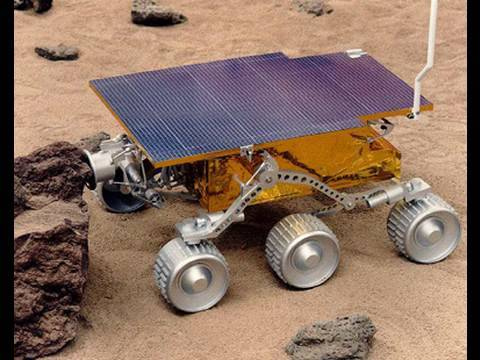
\includegraphics[width=2in]{misc_figs/pathfinder.png}
\end{center}
 

%\end{slide}

%\end{document}
























\chapter{USB}
    \input{USB.c.tex}

\end{document}

%  Use name of bibliography files without .bib extension
%\bibliography{brl}
\end{document}

